\chapter{System topology}
利用热力学原理进行定性分析。提炼出创新点。
\section{System topology design}
\subsection{Basic systems}

The objective of this research is to research the equipment of solar thermal power generation system, to propose, develop and optimize a solar thermal cascade system depending on the advantages and disadvantages of the solar thermal power generation systems. 
The research is based on the national cooperation project "Collaborative research on key technologies to produce electricity by cascade utilization solar thermal energy" as the background. 
There are three kinds of mature technologies been applied commercially -- parabolic trough, parabolic dish and solar tower. 
Considering the future deployment of solar cascade demo system, two solar thermal technologies, parabolic trough and parabolic dish, are chosen as the basic systems for the design of cascade solar thermal power system.
Figure~\

\begin{figure}[!ht]
\centering
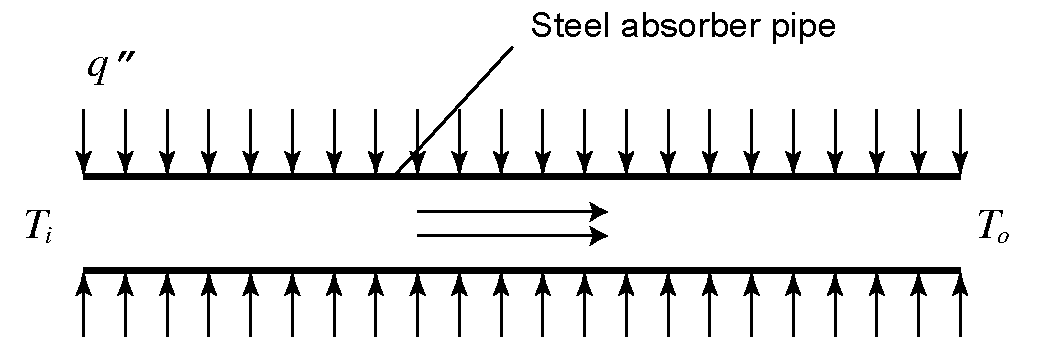
\includegraphics[width=0.6\textwidth]{fig/Pipe.pdf}
\caption{Schematic diagram of the absorber pipe}\label{fig:Pipe}
\end{figure}

\section{System topology selection}
各种拓扑结构分析

